\documentclass[10pt,twocolumn]{article}
\usepackage[a4paper,margin=1.8cm,columnsep=0.6cm]{geometry}
\usepackage[T1]{fontenc}
\usepackage{lmodern,microtype,graphicx,booktabs,array,amsmath,etoolbox,placeins,stfloats}
\usepackage[hidelinks]{hyperref}
\usepackage[font=small,labelfont=bf]{caption}
\setlength{\parskip}{3pt}\raggedbottom
\renewcommand{\arraystretch}{1.15}
% full-width figures are taller than the default 0.7 page limit; let them sit on top of a page
\renewcommand{\dbltopfraction}{0.95}\renewcommand{\dblfloatpagefraction}{0.85}\renewcommand{\textfraction}{0.05}\setcounter{dbltopnumber}{2}
\renewcommand{\topfraction}{0.9}\renewcommand{\bottomfraction}{0.8}\renewcommand{\floatpagefraction}{0.8}\setcounter{topnumber}{3}\setcounter{totalnumber}{5}

\title{Pretrained Decision Models in Bioinformatics:\\ Comparable to Active-Learning Screening, Baseline-Dependent in Cell-Type Annotation, Behind a Trained Mass-Spectrometry Re-scorer}
\author{%
  Mehmet Ali \"{O}zt\"{u}rk$^{1,2}$ \quad Simon Els\"{a}sser$^{1,2}$\\[6pt]
  {\small $^{1}$Institute for Biology, Universit\"{a}t Freiburg, Sch\"{a}nzlestrasse 1, 79104 Freiburg, Germany}\\
  {\small $^{2}$Center for Integrative Biological Signalling Studies (CIBSS), University of Freiburg,}\\
  {\small Sch\"{a}nzlestrasse 18, 79104 Freiburg, Germany}}
\date{}

\begin{document}
\twocolumn[\begin{@twocolumnfalse}
\maketitle
\begin{abstract}
Much of biomedical research rests on small, repeated decisions with a fixed set of answers: whether a study belongs in a systematic review, whether two trial claims contradict each other, which type a cell is, whether a peptide-spectrum match is correct. Pretrained decision models answer such questions without training on the data at hand, but how far they can replace the methods established for each task is unknown. Here we tested two such models, Jev and d3-ultra, against an established tool or, where none exists, published benchmark results, in four tasks with known answers, ordered from text input to numeric input. On text the models were usable without any training: in screening for 39 systematic reviews their reading order showed no detectable difference from the active-learning screener ASReview at the ideal stopping point, an upper bound because no reviewer knows that point in advance, and in detecting contradictory drug-trial claims they scored close to the best published model. On gene names they helped only where a curated marker database was weak: they trailed it in pancreas and led it in heart, by a margin that depended on how the database was applied. On numbers from one mass-spectrometry run they accepted 30 to 55\% fewer matches at 1\% estimated error than a re-scorer trained on that run. Pretrained decision models are therefore a practical first pass for text-based decisions and worth trying where curated knowledge is thin, but no substitute for a tool trained on the experiment's own numbers.
\end{abstract}\vspace{1.5em}
\end{@twocolumnfalse}]
\begin{figure*}[t]\centering
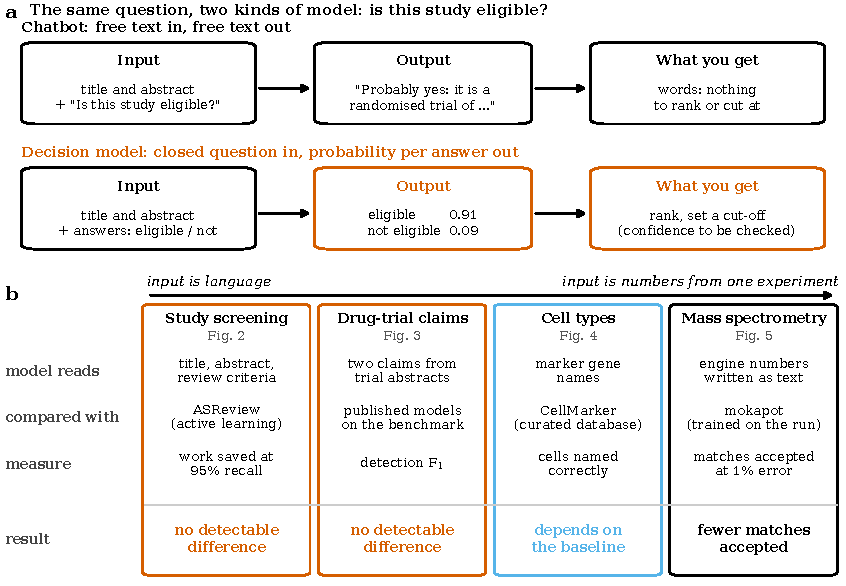
\includegraphics[width=\textwidth]{figs/fig1_gradient.pdf}
\caption{\textbf{What a decision model is, and the four tests.} \textbf{a}, The same question put to a chatbot and to a decision model: the chatbot answers in free text, the decision model returns a probability for each allowed answer (the example is the screening question). \textbf{b}, Four tests of Jev~1.13 and d3-ultra, ordered from text input to numeric input. Each column is one test, shown in full in the figure named under its title; rows give what the models read, what they are compared with and the primary measure. The bottom line is Jev's verdict: no detectable difference (orange), dependent on the baseline (light blue), or behind the comparator (black). Toward the right the input is numbers from one experiment and the comparator is trained on that experiment.}
\label{fig:gradient}
\end{figure*}

\section{Introduction}

Much of biomedical research is made of small decisions repeated many times, each with a fixed set of answers. An expert can make any one of them, but not at the scale the data now demand. A systematic review starts from thousands of titles and abstracts, of which a few percent are eligible~\cite{borah2017}, and each must be judged in or out. Trial reports appear at a rate that no reader can follow, and each apparent contradiction between them must be judged real or not before evidence can be pooled~\cite{bastian2010,ioannidis2005}. Single-cell atlases contain millions of cells, each of which must be given a type~\cite{tabula}, and a single proteomics run yields tens of thousands of peptide-spectrum matches, each to be judged correct or wrong~\cite{elias}. For each of these decisions the field has built a dedicated tool: active-learning screeners for reviews~\cite{asreview}, natural-language inference systems for claims~\cite{lan2026}, marker databases and reference classifiers for cell types~\cite{cellmarker,abdelaal}, and semi-supervised re-scorers for spectra~\cite{kall,mokapot}. Several of these tools, such as active-learning screeners, reference classifiers and re-scorers, learn from the data at hand, so they need labels or a run large enough to train on.

Pretrained decision models offer a different route. A decision model is a language model used for closed questions. Instead of writing a free answer like a chatbot, it is given a case and a fixed list of allowed answers and returns a probability for each (Fig.~\ref{fig:gradient}a)~\cite{jev,d3ultra}. A chatbot's reply is text that must be read or parsed and carries no number to rank by; a decision model's probabilities can order cases, be cut at a threshold and, if they are reliable, tell a researcher which answers to trust and which to check. The model is trained once, on a broad corpus, and is meant to judge cases it has never seen (zero-shot), so it needs no training on the task. Language models have been tried on several of these tasks one at a time~\cite{gptcelltype,guo2024,tabllm}, but single-task studies cannot show for which kinds of input such a model can stand in for a specialised tool.

Studies of decision models so far point to input type as a plausible factor. In medicine, Jev scored similarly to a frontier language model on questions about research abstracts but lower on examination questions and much lower on complex diagnostic cases~\cite{madrid2026}, and an open decision model came close to GPT-4 on medical examination questions but trailed supervised models on some predictions from patient records, where its probabilities were also poorly calibrated~\cite{medjev}. On biomedical text tasks with fixed choices Jev came close to general language models at under 1\% of their cost~\cite{chen2026}, it ranked records for systematic-review screening without labels~\cite{jo2026}, and on clinical diagnosis it matched frontier language models on short, distinctive complaints but fell well behind on patients with many symptoms~\cite{deobhakta2026}. Where the input is a signal or a measurement, such as EEG recordings~\cite{eegjev}, molecules~\cite{molrejev}, responses to genetic perturbation~\cite{s1pert} or ultrasound images~\cite{kevbio}, decision models have been trained or adapted on data of that kind rather than used as they come. A separate line of work gives language-model agents whole analyses to plan and run~\cite{drugcoding,omicsbench}; we look instead at the single, repeated decision inside such analyses. A model trained on language may handle text better than numbers from one experiment, whose scale it has never learned.

We address that question with four controlled tests of two pretrained decision models, Jev and d3-ultra, on public data with known answers. Three tests compare the models with the tool a practitioner would otherwise use; for drug-trial claims, where no dedicated tool was run, the two models are compared with each other and with the models published with the benchmark. The tasks span a gradient from text to numbers: study screening and claim comparison present natural text; cell-type annotation presents gene names, which are words that stand for measurements; peptide-spectrum re-scoring presents numbers written out as text (Fig.~\ref{fig:gradient}). The tasks also differ in comparator, benchmark and measure, so the gradient describes the tests rather than isolating input type.


\section{Approach}


\begin{figure*}[t]\centering
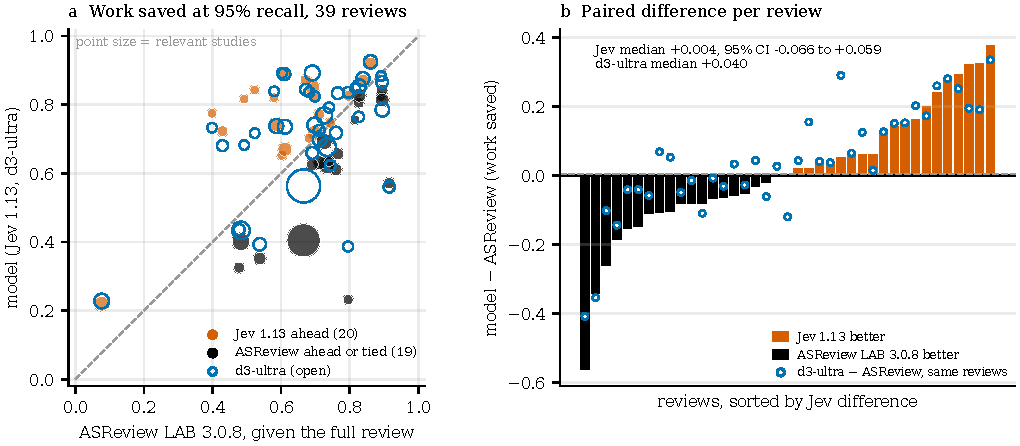
\includegraphics[width=\textwidth]{figs/fig2_screening.pdf}
\caption{\textbf{Screening: without training, the decision models order records with no detectable difference from ASReview.} Thirty-nine systematic reviews; Jev~1.13 and d3-ultra against ASReview LAB~3.0.8, scored on held-out records at the point where 95\% of eligible studies have been read.
\textbf{a}, Work saved per review, ASReview ($x$) against the models ($y$); point area scales with the number of eligible studies.
\textbf{b}, The same comparison as one paired difference per review, sorted; dashed line, median.}
\label{fig:screening}
\end{figure*}
Two pretrained decision models were tested, Jev~1.13~\cite{jev} and d3-ultra~\cite{d3ultra}. In drug claims they are compared with each other; in the other three tests d3-ultra is a second arm added after those studies closed. Each test sets the models against the tool a practitioner would otherwise use, on a public dataset with known answers, scored by one measure (Fig.~\ref{fig:gradient}b): work saved at 95\% recall for screening, F$_1$ for drug claims, accuracy for cell types, and matches accepted at 1\% estimated error for mass spectrometry. Where no such tool exists, as for drug claims, the models published with the benchmark take its place. Comparisons are paired, and a difference is called not detectable when its 95\% interval includes zero, which does not show that the two methods are equal. In the figures Jev is orange, d3-ultra blue, the specialised tool black and baselines without a model grey. Methods gives the questions, decision rules, data splits and statistics of each test.

\section{Results}
\subsection{Screening: no detectable difference from active learning}

A systematic review must find every study that meets its eligibility criteria, so the team reads the title and abstract of every record a literature search returns, often several thousand, of which only a few percent are eligible. Most of this reading is spent rejecting records, yet a missed eligible study can bias the review, so the convention is to find 95\% of the eligible studies while reading as few records as possible. Active-learning screeners such as ASReview~\cite{asreview} serve this goal today. The reviewer labels a few records, the screener trains a classifier on them, moves the records most likely to be eligible to the top of the list and retrains after each new label, so eligible studies turn up early. What the screener cannot tell the reviewer is when to stop. Nobody knows how many eligible studies remain unread, and the usual rule of thumb, a long run of rejected records, gives no guarantee of reaching 95\%.

A decision model needs neither labels nor training. Given a record's title and abstract and the review's eligibility criteria, it returns the probability that the record is eligible, and sorting the records by it gives a reading order from the first record on. We compared this order with ASReview LAB~3.0.8 on 39 completed reviews from SYNERGY+~\cite{synergy} whose eligible studies are known, scoring both methods on the same held-out records (18,183 records, 577 of them eligible). ASReview started, as in practice, from one eligible and one ineligible record, but was given every record of each review to learn from and learned the labels of the held-out records as it read them, which favours ASReview. The measure is work saved at 95\% recall~\cite{cohen2006}, the share of records a reviewer can leave unread while still finding 95\% of the eligible ones.

Without any training, the decision models' reading order showed no detectable difference from ASReview (Fig.~\ref{fig:screening}a). Jev saved a median 0.74 of the reading and ASReview 0.70, a paired difference of $+0.004$ (95\% interval $-0.066$ to $+0.059$); d3-ultra also saved 0.74 and saved slightly more than Jev in the paired comparison ($+0.024$, $+0.006$ to $+0.051$; Fig.~\ref{fig:screening}b). These savings are counted at the point where 95\% of the eligible studies have been read, which no reviewer can see in advance, so they are upper bounds for both methods. A decision model can instead be stopped at a cut-off set beforehand on each review's development records. With such a cut-off Jev found 550 of the 577 eligible studies, reached 95\% recall in 25 of the 39 reviews and saved a median 0.64, less than ASReview ($-0.057$, $-0.120$ to $-0.005$); d3-ultra stopped earlier, saving 0.67 but finding only 452 of the 577. With a few dozen eligible studies per review these per-review recalls are uncertain: for 13 of the 14 reviews in which Jev fell short, the 95\% interval of its recall still includes 0.95. For screening, a decision model can therefore produce a good reading order without the labelling that active learning needs, but a safe point to stop reading remains open for the model as for ASReview.

\subsection{Drug-trial claims: close to the best published model}
\begin{figure}[!b]\centering
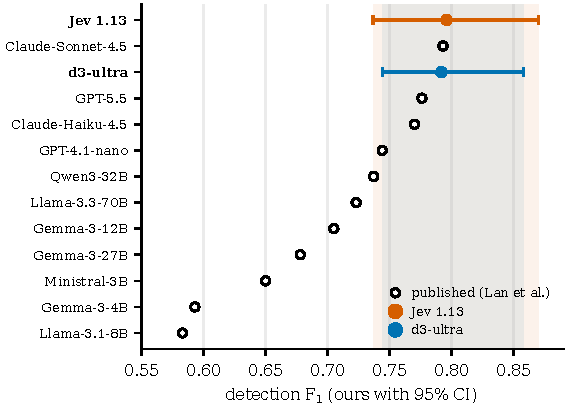
\includegraphics[width=\columnwidth]{figs/fig3_drug.pdf}
\caption{\textbf{Drug-trial claims: both decision models score close to the best published model.} Detection F$_1$ on the 1,731 expert-labelled pairs of DrugCon-Bench for Jev~1.13 and d3-ultra (95\% intervals from a bootstrap over the 217 abstract groups; shaded bands) beside the eleven models published with the benchmark (open circles; values from Lan et al.).}
\label{fig:drug}
\end{figure}

Contradictions between trial claims pose a second text problem. Before trial results can be pooled, evidence synthesis must know when two trials of the same drug in the same disease contradict each other, one claim reporting that the drug improved an outcome and the other that it did not or that it did harm. Most apparent contradictions dissolve once populations, doses, comparators or outcomes are compared~\cite{rothwell2005,alamri2016}, so each pair has to be read closely, and the number of pairs grows quickly with the number of trials. No established tool exists: reviewers compare claims by hand, and research systems treat the task as natural-language inference, deciding whether one statement contradicts another.

Without a tool to run, the baseline is a benchmark. DrugCon-Bench, released on 12 November 2026, holds 1,731 pairs of claims from randomised-trial abstracts, each labelled by expert annotators as contradictory or not (542 contradictory)~\cite{lan2026,lancode}. Its authors asked eleven general language models the question directly, and the best reached an F$_1$ of 0.793; F$_1$ balances finding contradictory pairs against raising false alarms, and 1 is perfect.

\begin{figure*}[b]\centering
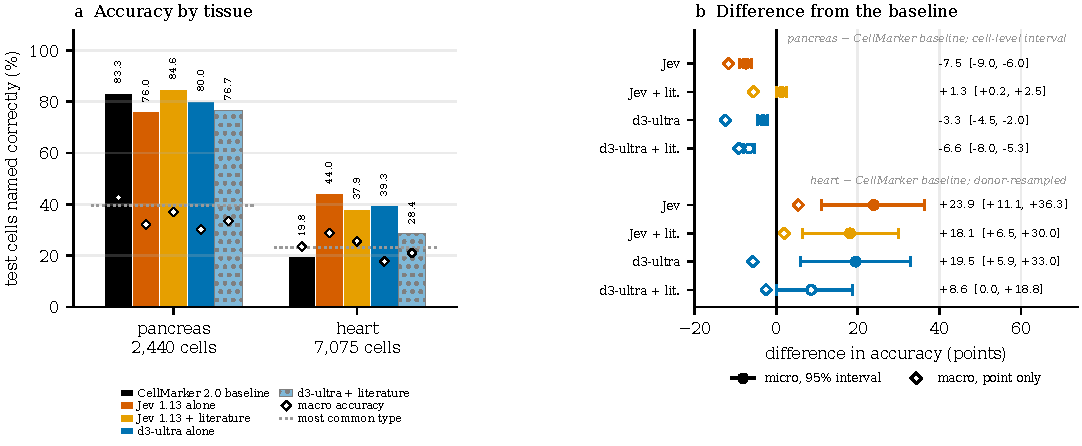
\includegraphics[width=\textwidth]{figs/fig4_cell.pdf}
\caption{\textbf{Cell types: Jev gains over CellMarker only where the database baseline is weak.} Held-out Tabula Sapiens cells.
\textbf{a}, Share of test cells named correctly (bars; Jev bars are means of three builds; blue, d3-ultra), macro accuracy (diamonds) and the share obtained by always naming the most common type (dotted). The baseline is the plain marker list in pancreas and the z-score version in heart; ``+ literature'' adds genes that PubMed articles mention together with each candidate gene.
\textbf{b}, Difference from the CellMarker baseline in accuracy (points, 95\% interval) and macro accuracy (open diamonds), first build. Heart intervals resample the six donors; pancreas intervals treat cells as independent and are too narrow.}
\label{fig:cell}
\end{figure*}

A decision model returns the probability that two claims contradict, and calling a pair contradictory when the model rates contradiction the more likely answer gives a verdict that can be scored like the published ones. Both decision models scored close to the best published model: Jev reached an F$_1$ of 0.796 (0.794 if the three pairs it rated at exactly one half are counted as contradictory), d3-ultra 0.792 and the best published model 0.793 (Fig.~\ref{fig:drug}). Close here means not detectably different, not ahead: of the eleven published models, Jev was detectably better than the six weakest and not detectably different from the other five, one of which, Qwen3-32B, lay at the edge (interval from $-0.0004$); d3-ultra was detectably better than the same six, Qwen3-32B and, at the edge, GPT-4.1-nano (interval from $+0.0002$), and not detectably different from the other three. These intervals treat the published scores as fixed, because only summary values are available, so they are somewhat too narrow. The probabilities themselves were informative beyond the verdict. They ranked contradictory pairs above the others (area under the ROC curve 0.941 for Jev and 0.931 for d3-ultra, where 1 is a perfect ranking) and lay close to the observed frequencies, on average 0.06 away for Jev and 0.09 for d3-ultra. The reference labels were seeded by one of the published models, GPT-4.1-nano: annotators confirmed 494 of the 615 pairs it flagged, and reviewing every remaining candidate pair in the same 819 abstracts added 48. For evidence synthesis, a decision model can therefore flag contradicting claim pairs with no detectable difference from the best general language models, leaving the expert to confirm the flagged pairs.

\subsection{Cell types: a gain only where the database is weak}

\begin{figure*}[t]\centering
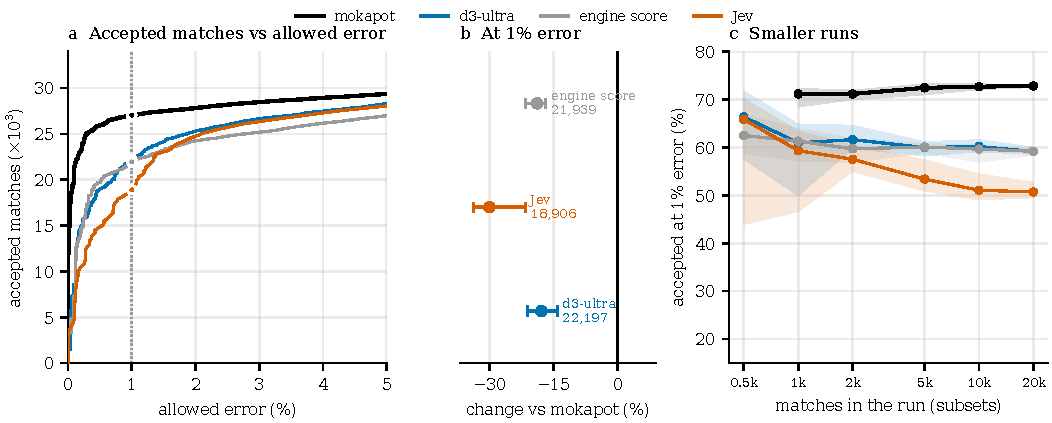
\includegraphics[width=\textwidth]{figs/fig5_massspec.pdf}
\caption{\textbf{Mass spectrometry: the decision models accept fewer matches than a re-scorer trained on the run.} Re-scoring 37,061 peptide-spectrum matches of one human run.
\textbf{a}, Accepted matches as the allowed error rises; dots mark the 1\% level used in the text.
\textbf{b}, Accepted matches at 1\% error relative to mokapot~0.10.0 (vertical line), with 95\% bootstrap intervals and counts.
\textbf{c}, Accepted share at 1\% error in random subsets of the run (20 per size; median and interquartile range); mokapot could not be trained on any subset of 500 matches and on 12 of the 20 subsets of 1,000, where it failed or fell back to a single engine number.}
\label{fig:massspec}
\end{figure*}

Cell-type annotation sits halfway along the gradient, because its input is gene names, each standing for an expression measurement. After single-cell RNA sequencing every cell must be named, and a common route uses marker genes, genes whose activity is typical of one cell type: a cell that expresses the markers of a type receives that type's name. Classifiers trained on an annotated reference of the same tissue name cells best, but need such a reference. Without one, analysts take marker lists from curated databases such as CellMarker~2.0~\cite{cellmarker}, collected from the literature; such lists are only as complete as the literature behind them, and their coverage differs between tissues.

A decision model has read the same literature. For each candidate gene we asked Jev which of the tissue's cell types the gene marks; its answers, one probability per type, form a marker list built without a reference and without curation. Both lists were then used in the same way: each cell receives the type whose marker genes it expresses most strongly. The test cells were expert-annotated cells held out from the Tabula Sapiens atlas~\cite{tabula}, 2,440 from pancreas, a tissue the database covers well, and 7,075 from heart, one it covers poorly. The measure is accuracy, the share of cells given the same name as the experts gave them.

In pancreas the database remained the better choice. Because both lists were used the same way, only the lists differ, and the database named 81.8\% of cells correctly against 75.6\% for Jev (Fig.~\ref{fig:cell}a,b): about six more cells in every hundred received the right name from the curated lists. With each cell type counted equally, Jev's list scored 41.4\% against 39.5\% for the same database lists, and the z-score version of the database described below scored 53.6\%, above both.

Heart shows what the model can add where curated markers are thin. The database lists, applied as in pancreas, named almost no heart cells correctly, so we compared the models with two ways an analyst would repair the database. Standardising each gene's expression across the cells before scoring (the z-score version) named 19.8\% of heart cells. Dividing each type's score by the length of its marker list (the size-normalised version, tried after the results were known) named 26.8\%. With neither repair, Jev's list named 48.1\% of heart cells (the average of three builds of the list) and d3-ultra's named 41.0\% (Fig.~\ref{fig:cell}a,b).

Both models thus named more heart cells than either version of the database. To see how firm that lead is, we resampled the six donors the heart cells come from, which gives approximate 95\% intervals~\cite{field2007}, for Jev from the first build. Against the z-score version the lead was detectable for both models: 28.1 points for Jev ($+16.7$ to $+42.1$) and 21.2 points for d3-ultra ($+7.5$ to $+35.9$). Jev's lead was also detectable with each cell type counted equally, however many cells it has (34.6\% against 23.4\%, a gain of 11.2 points, $+5.0$ to $+13.6$), whereas d3-ultra then showed no detectable difference from the z-score version (20.6\% against 23.4\%). Against the size-normalised version Jev's lead was not detectable, counted over cells ($+21.1$ points, $-0.2$ to $+37.6$) or over cell types ($+4.3$ points, $-2.4$ to $+8.0$). A decision model is therefore worth trying where curated markers are thin, not where a good database exists, and its gain should be judged against the best way of applying the database, not only the default one.

\subsection{Mass spectrometry: behind a re-scorer trained on the run}

Mass spectrometry closes the gradient with an input of numbers only. In shotgun proteomics a search engine matches each recorded spectrum to its best candidate peptide and reports numbers that describe the fit, such as a match score and a mass error. Many matches are wrong, so laboratories accept matches only down to a chosen estimated error rate, here 1\%. The rate is usually estimated from decoy peptides, sequences known to be absent~\cite{elias}; here we estimated it by entrapment~\cite{wen}. The search database also held the proteins of a plant, \emph{Arabidopsis thaliana}, absent from the human sample, so every match to a plant-only peptide is known to be wrong, and their count, scaled by the relative size of the plant and human databases, estimates the number of wrong matches. At a fixed error rate, more accepted matches means more peptides identified from the same run. Re-scorers such as Percolator and its reimplementation mokapot~\cite{kall,mokapot} raise this number: they train a small classifier on each run, using the decoy matches as examples of wrong matches, and combine the engine's numbers into one better score, provided the run is large enough to train on.

A decision model needs no training and so works on a run of any size. We wrote each match as one line listing the numbers the search engine reports, and the model returned the probability that the match is correct; both models received the same questions. Mokapot on the same run was the baseline, and the search engine's own score a lower reference that any re-scorer should beat. The run was one human sample with 37,061 matches~\cite{chick}, searched with Sage~\cite{sage}; each method's matches were accepted down to 1\% estimated error and counted.

The decision models accepted far fewer matches than mokapot: mokapot kept 27,047, Jev 18,906 (30.1\% fewer) and d3-ultra 12,157 (55.1\% fewer), both below the 21,939 kept by the search engine's own score (Fig.~\ref{fig:massspec}a,b). Small runs, where mokapot cannot be trained, were the one setting in which a model without training could have helped, but there too the decision models did not accept reliably more matches than the engine's score (Fig.~\ref{fig:massspec}c). A classifier trained on the run with only the numbers the models saw kept 27,071 matches, no detectable difference from mokapot ($+0.1\%$, 95\% interval $-0.5$ to $+0.5$), so the input sufficed. The models did not help mokapot either: given a model's probability as one more feature, mokapot kept 27,047 matches with Jev ($+0.0\%$, $-0.2$ to $+0.5$) and 27,021 with d3-ultra ($-0.1\%$, $-0.4$ to $+0.2$), no detectable difference from mokapot alone. For proteomics, a re-scorer trained on the run remains the tool of choice.

\begin{table*}[t]\centering\small
\caption{\textbf{The four tests at a glance.} One headline number per test, Jev against the comparator; intervals and the d3-ultra results are in the Results.}
\label{tab:summary}
\begin{tabular}{@{}>{\raggedright}p{2.2cm}>{\raggedright}p{2.8cm}>{\raggedright}p{2.8cm}>{\raggedright}p{3.4cm}>{\raggedright\arraybackslash}p{3.5cm}@{}}
\toprule
Task & The model reads & Compared with & Headline & Take-home\\
\midrule
Study screening & title, abstract, review criteria & ASReview, an active-learning screener & work saved 0.74 vs 0.70 & no detectable difference at the ideal stopping point, without training\\
Drug-trial claims & two claims from trial abstracts & published models on the benchmark & F$_1$ 0.796 (Jev) and 0.792 (d3-ultra) vs best published 0.793 & close to the best published model\\
Cell types & marker gene names & CellMarker 2.0, a curated database & cells named correctly: pancreas 75.6\% vs 81.8\%; heart 48.1\% vs 19.8\% & behind where the database is good; where it is weak, ahead of its usual use, but no detectable difference from a stronger use\\
Mass spectrometry & match scores written as text & mokapot, trained on the run & 30 to 55\% fewer accepted matches at 1\% error & behind a trained re-scorer\\
\bottomrule
\end{tabular}
\end{table*}

\section{Discussion}

We asked how far a pretrained decision model can stand in for a specialised tool. In these four tests the results lined up with the input (Table~\ref{tab:summary}). On text the models were usable without training: their reading order for screening showed no detectable difference from active learning at the ideal stopping point, and their verdicts on trial claims came close to the best published model. On gene names they helped only where curated knowledge was thin. On numbers from one experiment they fell well behind a re-scorer trained on that experiment. The comparators change along the same axis, being trained on the run itself toward the numeric end, so the ordering describes these four tests rather than isolating input type.

Earlier studies tested language models on single tasks: reading abstracts for screening~\cite{guo2024}, annotating cell types from marker genes~\cite{gptcelltype}, and classifying tabular data~\cite{tabllm,hollmann}. Setting four tasks side by side, each against the tool a practitioner would use, suggests a pattern that no single test can show: in these tests, the further the input moved from language toward measurements, the less a model trained on language added. The heart result also shows how much such comparisons depend on the comparator: a gain over a weak baseline shrank against a stronger one.

Other evaluations of decision models fit this pattern. Two are closest to our text cases. Jo et al.\ ranked screening records with Jev without labels and found it ahead of a free ranker, while stopping safely still required screening decisions~\cite{jo2026}, the open question our screening result leaves; their reviews and protocol differ from ours, so the numbers are not comparable. Chen et al.\ found Jev competitive with general language models on biomedical text tasks with fixed choices~\cite{chen2026}. Where the input demands more synthesis, decision models fell behind: Jev trailed frontier language models on diagnosis from many symptoms~\cite{deobhakta2026} and on complex diagnostic cases~\cite{madrid2026}, and an open decision model trailed supervised models on some predictions from patient records~\cite{medjev}, much as our models trailed the trained re-scorer on spectra. On patient records the open model's probabilities were also poorly calibrated until a recalibration fitted on 50 to 200 local examples corrected them~\cite{medjev}; a small amount of local fitting of this kind may also narrow the gap on numeric inputs, which we did not test. Studies that reached signals and measurements trained or adapted a decision model on such data~\cite{eegjev,molrejev,s1pert,kevbio}, consistent with our finding that a model used as it comes falls behind a re-scorer trained on the run.

The four tests also suggest how such a model is best used. In each, the model made one narrow decision inside an existing analysis (which record to read next, whether two claims conflict, which cell type a gene marks, whether a match is correct) and was judged against the tool that step normally uses; a model that falls short is then caught by the comparison before it changes a result. The check matters for a second reason: decision models can be swayed by wording. When irrelevant labels or pressure cues were added to clinical cases, decision models changed 13.4 more decisions per 100 than with neutral wording, and a language model 14.0, while pairing the two reduced these changes~\cite{omar2026}. The same step-by-step check fits agents that plan and run whole bioinformatics analyses, which still fail at many steps~\cite{omicsbench}: a decision model checked against the usual tool for one step could be one of the tools they call~\cite{drugcoding}.

The tests share limits. Each rests on one version of each model and one dataset per task, and the comparators and measures differ between tasks, so the results may not carry over to other models or data. The mass-spectrometry result comes from one run; its intervals resample matches within that run and do not capture variation between runs or laboratories. The more serious limit is possible data leakage. The decision models were trained on large text collections whose content is not disclosed, while most of what was tested is public: the screening reviews and their inclusion decisions, the trial abstracts, and the literature and databases from which marker lists are built. Part of what looks like judgement may therefore be recall of answers seen during training~\cite{sainz}. We did not test for this, and if present, it would inflate the text and gene-name results most, because that is where such material is most likely to have been seen. One partial check exists: the DrugCon-Bench labels were released on 12 November 2026, and although both models answered the drug-claim questions on 20 November, the Jev version used was already answering our questions in early October, so Jev is unlikely to have been trained on the labels, provided the version name marks a fixed model; the abstracts themselves were public, and for d3-ultra no such date is known. Some analysis choices were made after the results were known, and d3-ultra was added after the source studies had closed, so all results are exploratory. In five screening reviews the test records had been seen while the method was developed; leaving these reviews out did not change the Jev--ASReview comparison ($+0.002$, $-0.066$ to $+0.061$). d3-ultra was queried on 1,792 held-out screening records before its cut-off was set; those answers were not used to set it.
The comparators are also not exhaustive: we did not run a dedicated cell-type annotation tool, a model trained to compare claims, or re-scorers other than mokapot, and we did not test whether rewording the questions changes the answers.

For the many small judgements biomedical research depends on, a pretrained decision model is worth trying where the input is text or where curated knowledge is thin, provided it is compared with the user's usual tool on the user's own task. Where the input is numbers from one experiment large enough to train on, a tool trained on that experiment remains the better choice.

\section{Methods}

\subsection{Decision models and queries}
Two decision models were used, Jev~1.13 (TypeSafe System One~\cite{jev}) and d3-ultra (vLLM Semantic Router~\cite{d3ultra}), both through their web services and with the same requests. A request describes the case in short text fields and asks one or more questions, each with a fixed set of allowed answers. The model returns a probability for each allowed answer, or a score between 0 and 1. Neither service offers settings such as a temperature or a random seed, and repeated calls gave stable answers: asked twice, 200 drug-claim pairs received the same verdict in 99.5\% of cases from Jev and in all cases from d3-ultra. The tests were first run with Jev, and d3-ultra was added afterwards with the same questions. All answers were stored, so every result can be rebuilt without calling the models again. The exact questions, a worked example for each test and the code are in the repository.

\subsection{Study screening}
The data were 39 systematic reviews from SYNERGY+~\cite{synergy}, each with titles, abstracts, eligibility criteria and final inclusion decisions. The records of each review were split at random into parts for development and for testing, and all results come from the test parts (18,183 records, 577 of them eligible). For each record the models read the title, the abstract and the review's eligibility criteria and scored whether the record should go on to full-text review. This score ordered the records. The pre-set cut-off of a review was the highest score that still found 95\% of the eligible studies among its development records, and it was applied unchanged to the test records.

The comparator was ASReview LAB~3.0.8~\cite{asreview}, run once per review in simulation mode from one eligible and one ineligible record. The measure is work saved at 95\% recall~\cite{cohen2006}: the share of records left unread at the point where 95\% of the eligible records have been found, minus 0.05.

\subsection{Drug-trial claims}
DrugCon-Bench~\cite{lan2026} pairs claims from randomised-trial abstracts on the same drug and disease. It holds 1,731 pairs, of which 542 contradict each other. The benchmark's labels started from pairs flagged by one of the published models, which annotators then checked and extended. Each pair was put to the models as one question with two answers, that the claims contradict or that they can coexist, worded after the benchmark authors' own prompt. A pair was called contradictory when that answer had the higher probability, a rule fixed before any run. The measure is F$_1$ for the contradictory pairs, computed with the authors' evaluation code. The scores of the eleven published models were taken from the benchmark paper, using for each model the better of its two prompts. They were published without intervals and are treated as fixed values.

\subsection{Cell types}
Expert-annotated cells of pancreas and heart came from Tabula Sapiens~\cite{tabula}, and a fifth of each cell type was held out for testing (2,440 pancreas and 7,075 heart cells). The candidate genes were the CellMarker~2.0~\cite{cellmarker} markers of each tissue's cell types. For each gene the models were asked which of the tissue's cell types it marks, or none of them, and the returned probabilities form a table of genes by cell types that takes the place of the database list. Each cell then received the type whose marker genes carried the largest share of its expression, by the same rule for the model and database lists.

Applied in this way, the database list assigned almost all heart cells to one type, so for heart it was also scored in two further ways. The z-score version standardises each gene's expression across the test cells before scoring. The size-normalised version, added after the first results were seen, divides each type's score by the number of genes listed for it. Each model built its list three times; the text reports the average, and comparisons with the database use Jev's first build. Figure~\ref{fig:cell} also shows a second arm in which genes often mentioned together with each gene in the literature were added to the question.

\subsection{Mass spectrometry}
One run of a human cell line from a public dataset~\cite{chick} was searched with Sage~\cite{sage}, using standard tryptic settings, against the human proteins together with the proteins of a plant, \emph{Arabidopsis thaliana}, which cannot be in the sample. The search gave 37,061 matches to real sequences. Each match was put to the models as one yes-or-no question listing the search engine's numbers for that match, such as scores, mass errors, matched fragments and explained signal. The models never saw the peptide sequence, the species or any re-scorer output, and the probability of ``yes'' ranked the matches.

The comparator was mokapot~0.10.0~\cite{mokapot}, trained on the run with its standard inputs. Two further checks used the same run: a classifier trained on only the numbers the models saw, and mokapot given each model's probability as one more input. For the small-run test, mokapot was retrained on random subsets of 500 to 20,000 matches, 20 per size.

The error among accepted matches was estimated by entrapment~\cite{wen}. A match to a plant protein must be wrong, so the number of such matches, scaled for the sizes of the two protein sets, estimates how many accepted human matches are wrong. Each method's matches were accepted down to the score at which this estimate reached 1\%.

All comparisons are paired. Intervals are 95\% bootstrap intervals, obtained by resampling the unit that carries the dependence: the review for screening, the group of pairs that share abstracts for drug claims, the donor for heart (approximate with only six donors~\cite{field2007}) and the match for mass spectrometry. The pancreas data carry no donor labels, so that interval was computed over cells. A difference is called not detectable when its interval includes zero, which does not show that the methods are equal. Intervals are descriptive and were not adjusted for the number of comparisons. The stored results behind every comparison, and the code that computes its interval, are in the repository.
All comparisons are paired. Intervals are 95\% bootstrap intervals, obtained by resampling the unit that carries the dependence: the review for screening, the group of pairs that share abstracts for drug claims, the donor for heart (approximate with only six donors~\cite{field2007}) and the match for mass spectrometry. The pancreas data carry no donor labels, so that interval was computed over cells. A difference is called not detectable when its interval includes zero, which does not show that the methods are equal. Intervals are descriptive and were not adjusted for the number of comparisons. The values and intervals of every comparison are in the repository.


\section*{Acknowledgements}
This work was supported by the Claude AI for Science program (Anthropic).

\section*{Data and code availability}
Raw files larger than 50\,MB (mass-spectrometry spectra, single-cell expression files) are listed with size and checksum for download rather than shipped. Data, code and paper source: \url{https://github.com/oeztuerkmehmetali-del/decision-model-benchmark}.

\begin{thebibliography}{99}\small
\bibitem{borah2017} Borah R, Brown AW, Capers PL, Kaiser KA. Analysis of the time and workers needed to conduct systematic reviews of medical interventions using data from the PROSPERO registry. \emph{BMJ Open} 7:e012545 (2017). doi:10.1136/bmjopen-2016-012545
\bibitem{bastian2010} Bastian H, Glasziou P, Chalmers I. Seventy-five trials and eleven systematic reviews a day: how will we ever keep up? \emph{PLoS Med} 7:e1000326 (2010). doi:10.1371/journal.pmed.1000326
\bibitem{ioannidis2005} Ioannidis JPA. Contradicted and initially stronger effects in highly cited clinical research. \emph{JAMA} 294:218--228 (2005). doi:10.1001/jama.294.2.218
\bibitem{tabula} Tabula Sapiens Consortium. The Tabula Sapiens: a multiple-organ, single-cell transcriptomic atlas of humans. \emph{Science} 376:eabl4896 (2022). doi:10.1126/science.abl4896
\bibitem{elias} Elias JE, Gygi SP. Target-decoy search strategy for increased confidence in large-scale protein identifications by mass spectrometry. \emph{Nat Methods} 4:207--214 (2007). doi:10.1038/nmeth1019
\bibitem{asreview} van de Schoot R, et al. An open source machine learning framework for efficient and transparent systematic reviews. \emph{Nat Mach Intell} 3:125--133 (2021). doi:10.1038/s42256-020-00287-7
\bibitem{lan2026} Lan M, Menke J, Liu S, Lu Z, Kilicoglu H. Detecting contradictory evidence on drug-disease associations at scale. \emph{medRxiv} (preprint, not peer reviewed), 12 Nov 2026. doi:10.64898/2026.11.11.26367856
\bibitem{cellmarker} Hu C, et al. CellMarker 2.0: an updated database of manually curated cell markers in human/mouse and web tools based on scRNA-seq data. \emph{Nucleic Acids Res} 51:D870--D876 (2023). doi:10.1093/nar/gkac947
\bibitem{abdelaal} Abdelaal T, et al. A comparison of automatic cell identification methods for single-cell RNA sequencing data. \emph{Genome Biol} 20:194 (2019). doi:10.1186/s13059-019-1795-z
\bibitem{kall} K\"all L, Canterbury JD, Weston J, Noble WS, MacCoss MJ. Semi-supervised learning for peptide identification from shotgun proteomics datasets. \emph{Nat Methods} 4:923--925 (2007). doi:10.1038/nmeth1113
\bibitem{mokapot} Fondrie WE, Noble WS. mokapot: fast and flexible semisupervised learning for peptide detection. \emph{J Proteome Res} 20:1966--1971 (2021). doi:10.1021/acs.jproteome.0c01010
\bibitem{jev} TypeSafe AI. Jev (System One model) documentation. Model used: \texttt{jev-1.13.0}. \url{https://docs.typesafe.ai} (accessed 20 Nov 2026).
\bibitem{d3ultra} vLLM Semantic Router project. d3-ultra (decision model). Hugging Face (2026). \url{https://huggingface.co/vllm-sr/d3-ultra} (accessed 23 Nov 2026).
\bibitem{gptcelltype} Hou W, Ji Z. Assessing GPT-4 for cell type annotation in single-cell RNA-seq analysis. \emph{Nat Methods} 21:1462--1465 (2024). doi:10.1038/s41592-024-02235-4
\bibitem{guo2024} Guo E, Gupta M, Deng J, Park YJ, Paget M, Naugler C. Automated paper screening for clinical reviews using large language models: data analysis study. \emph{J Med Internet Res} 26:e48996 (2024). doi:10.2196/48996
\bibitem{tabllm} Hegselmann S, et al. TabLLM: few-shot classification of tabular data with large language models. In \emph{Proc.\ AISTATS}, PMLR 206:5549--5581 (2023). arXiv:2210.10723
\bibitem{madrid2026} Madrid-Garc\'{\i}a A, Merino-Barbancho B. Jev in Medicine: a benchmark evaluation. \emph{arXiv} 2609.34024 (2026). doi:10.48550/arXiv.2609.34024
\bibitem{medjev} Lee SA, Sha J, Jeong M, Pan Y, Chiang JN. MedJev: evaluating zero-shot System-One decision making in medicine. \emph{arXiv} 2610.36006 (2026). doi:10.48550/arXiv.2610.36006
\bibitem{chen2026} Chen AF, Yang A, Guth DR, Berl FM, Guth SC, Yuan W. Evaluation of System One models on biomedical texts. \emph{medRxiv} (preprint, not peer reviewed), 17 Nov 2026. doi:10.64898/2026.11.15.26368126
\bibitem{jo2026} Jo T, Lee D, Lee L. Label-free, low-cost AI ranking for systematic review screening. \emph{medRxiv} (preprint, not peer reviewed), 19 Oct 2026. doi:10.64898/2026.10.09.26365173
\bibitem{deobhakta2026} Deobhakta A, Chang JS, Chen RWS, Jaipalli S, Pinhas A, Tai TYT, Rosen R. Do calibrated-probability claims hold up in clinical diagnosis? A pre-registered evaluation of a decision model against frontier language models. \emph{medRxiv} (preprint, not peer reviewed), 11 Oct 2026. doi:10.64898/2026.10.09.26365153
\bibitem{eegjev} Hou D, Yamada KD. EEGJev: a System One decision model and benchmark for multi-task EEG question answering. \emph{arXiv} 2611.32100 (2026). doi:10.48550/arXiv.2611.32100
\bibitem{molrejev} Lu K, Li J, Bian Y. MolReJev: decision models are in-context molecular predictors. \emph{arXiv} 2611.28965 (2026). doi:10.48550/arXiv.2611.28965
\bibitem{s1pert} Sheng X, et al. S1Pert: scalable target-specific gene response prediction with System-One intelligence. \emph{arXiv} 2611.17705 (2026). doi:10.48550/arXiv.2611.17705
\bibitem{kevbio} Heidari M, et al. Every pixel is an option: a System One model for medical ultrasound biometry. \emph{arXiv} 2611.03360 (2026). doi:10.48550/arXiv.2611.03360
\bibitem{drugcoding} Hu J, Lin Z, Li K, Zhang H. DrugCoding: a scientific programming agent for drug discovery. \emph{arXiv} 2611.13651 (2026). doi:10.48550/arXiv.2611.13651
\bibitem{omicsbench} Shaked G, Nagisetty S. OmicsBench: a long-horizon multi-turn benchmark of AI agents on research-study-scale bioinformatics. \emph{arXiv} 2610.21074 (2026). doi:10.48550/arXiv.2610.21074
\bibitem{synergy} De Bruin J, et al. SYNERGY dataset v1.0. doi:10.34894/HE6NAQ; Westerbeek E, et al. SYNERGY+ v3.0. doi:10.34894/ddcvcv.
\bibitem{cohen2006} Cohen AM, Hersh WR, Peterson K, Yen PY. Reducing workload in systematic review preparation using automated citation classification. \emph{J Am Med Inform Assoc} 13:206--219 (2006). doi:10.1197/jamia.M1929
\bibitem{rothwell2005} Rothwell PM. External validity of randomised controlled trials: ``To whom do the results of this trial apply?'' \emph{Lancet} 365:82--93 (2005). doi:10.1016/S0140-6736(04)17670-8
\bibitem{alamri2016} Alamri A, Stevenson M. A corpus of potentially contradictory research claims from cardiovascular research abstracts. \emph{J Biomed Semantics} 7:36 (2016). doi:10.1186/s13326-016-0083-z
\bibitem{lancode} Lan M. DrugCon\_Drug\_Contradiction (code and data). GitHub (2026), commit 2c2d5f5.
\bibitem{field2007} Field CA, Welsh AH. Bootstrapping clustered data. \emph{J R Stat Soc B} 69:369--390 (2007). doi:10.1111/j.1467-9868.2007.00593.x
\bibitem{wen} Wen B, et al. Assessment of false discovery rate control in tandem mass spectrometry analysis using entrapment. \emph{Nat Methods} 22:1454--1463 (2025). doi:10.1038/s41592-025-02719-x
\bibitem{chick} Chick JM, et al. A mass-tolerant database search identifies a large proportion of unassigned spectra in shotgun proteomics as modified peptides. \emph{Nat Biotechnol} 33:743--749 (2015). doi:10.1038/nbt.3267
\bibitem{sage} Lazear MR. Sage: an open-source tool for fast proteomics searching and quantification at scale. \emph{J Proteome Res} 22:3652--3659 (2023). doi:10.1021/acs.jproteome.3c00486
\bibitem{hollmann} Hollmann N, et al. Accurate predictions on small data with a tabular foundation model. \emph{Nature} 637:319--326 (2025). doi:10.1038/s41586-024-08328-6
\bibitem{omar2026} Omar M, Ramaswamy A, Sakhuja A, et al. Decision-only medical AI: early evidence and pairing with language models. \emph{medRxiv} (preprint, not peer reviewed), 24 Oct 2026. doi:10.64898/2026.10.21.26366149
\bibitem{sainz} Sainz O, et al. NLP evaluation in trouble: on the need to measure LLM data contamination for each benchmark. In \emph{Findings of EMNLP}, 10776--10787 (2023). arXiv:2310.18018
\end{thebibliography}
\end{document}
